%!TEX root=../../autopilot.tex
\section{Distributed Go/No-go Task}
\label{sec:gonogo}

\begin{margintable}[-1.5cm]
\caption{Go/No-go Materials}
\label{tab:gonogomat}
\noindent\begin{tabularx}{\linewidth}{lX}%
\toprule
\textbf{Hardware} & \\
\textbf{Beam Break} & \href{https://wiki.auto-pi-lot.com/index.php/TT_Electronics_OPB901L55}{TT Electronics OPB901L55} \\
\textbf{Monitor} & \href{https://www.productchart.com/monitors/16901}{Acer S230HL} \\
\textbf{Lick Port} & \href{https://wiki.auto-pi-lot.com/index.php/Autopilot_Tripoke}{Autopilot Tripoke v1} \\
\textbf{Light Sensor} & \href{https://www.thorlabs.com/newgrouppage9.cfm?objectgroup_id=3341}{Thorlabs PM100D} \\
\midrule
\textbf{Software} & \\
\textbf{psychopy} & v3.1.5 \\
\textbf{glfw} & v1.8.3 \\
\bottomrule
\end{tabularx}
\end{margintable}{}

We designed a visual go/no-go task as a proof of concept for distributing task elements across multiple Pis, and also for the presentation of visual stimuli (Figure \ref{fig:gonogo}, Table \ref{tab:gonogomat}). The code for this task is described in greater detail in \href{https://wiki.auto-pi-lot.com/index.php/Plugin:Autopilot_Paper}{the wiki page} for the plugin that accompanies this paper. While the rest of the tests presented have been re-run, in the time since the intitial publication of the preprint we have not done substantial work on Autopilot's visual stimulus module, and so this section is presented as previously written using the v0.1.0 initial release.

\begin{marginfigure}[-0cm]
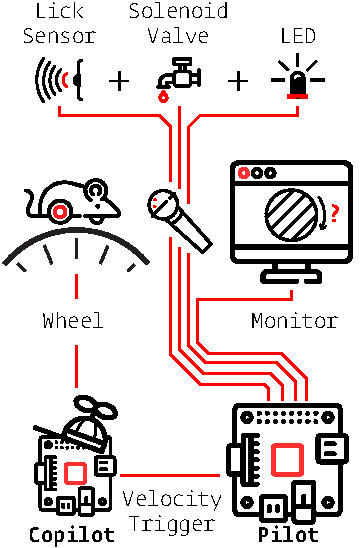
\includegraphics[]{figures/test_5_gonogo.pdf}
\caption{Hardware distribution for the distributed go/no-go task. Red lines indicate physical connections between hardware components. The lick sensor, solenoid valve, and LED are physically bundled into one component represented as the mouse's microphone.}
\label{fig:gonogo}
\end{marginfigure}

In this task, a head-fixed subject would\sidenote{No mice were trained on this task} be running on a wheel in front of a display with a lick-detecting water port able to deliver reward. Above the port is an LED. Whenever the LED is green, if the subject drops below a threshold velocity for a fixation period, a grating stimulus at a random orientation is presented on the monitor. After a random delay, there is a chance that the grating changes orientation by a random amount. If the subject licks the port in trials when the orientation is changed, or refrains from licking when it is not, the subject is rewarded. 

One pilot controlled the operation of the task, including the coordination of a copilot. The pilot was connected to the LED and solenoid valve for reward delivery, as well as a monitor\sidenote{(\texttt{1920x1080px, 60Hz})} to display the gratings\sidenote{Visual stimuli were presented with \href{https://www.psychopy.org/}{Psychopy} using the \href{https://www.glfw.org/}{glfw} backend while Autopilot was run in a dedicated X11 server.}. The copilot continuously streamed velocity data (measured with a USB optical mouse against the surface of the wheel) back to the terminal for storage (see also Figure \ref{fig:datastreams}, which depicts the network topology for this task). The copilot waited for a message from the pilot to initiate measuring velocity, and when a rolling average of recent velocities fell below a given threshold the copilot sent a TTL trigger back to the pilot to start displaying the grating. This split-pilot topology allows us to poll the subject velocity continuously (at \texttt{125Hz} in this example) without competing for resources with psychopy's rendering engine.

We measured trigger (TTL pulse from the copilot) to visual stimulus onset latency using the measurement cursors of our oscilloscope as before. To detect the onset of the visual stimulus, we used a high-speed optical power meter attached to the top-left corner of our display monitor. The stimulus was a drifting Gabor grating drawn to fill half the horizontal and vertical width of the screen (\texttt{960 x 540px}), with a spatial frequency of \texttt{4cyc/960px} and temporal (drift) frequency of \texttt{1Hz}.

\begin{marginfigure}[-0cm]
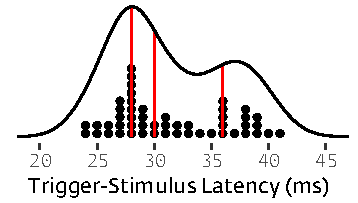
\includegraphics[]{figures/test_6_visual_lags.pdf}
\caption{Stacked dots are a histogram of individual observations (n=50) underneath the probability density (black line), red lines indicate quartiles.}
\label{fig:vidlat}
\end{marginfigure}

We observed a bimodal distribution of latencies (Quartiles: \texttt{28, 30, 36ms, n=50}, Figure \ref{fig:vidlat}), presumably because onsets of visual stimuli are quantized to the refresh rate (\texttt{60Hz, 16.67ms}) of the monitor. This range of latencies corresponds to the second and third frame after the trigger is sent (2/3 of observations fall in the 2nd frame, 1/3 of observations in the 3rd frame). We observed a median framerate of \texttt{36.2 FPS (IQR: 0.7)} across 50 trials (\texttt{8863} frames, Figure \ref{fig:framerate}). 

We further tested the Pi's framerate by using Psychopy's \href{https://github.com/psychopy/psychopy/blob/3.1/psychopy/demos/coder/timing/timeByFrames.py}{\texttt{timeByFrames}} test---a script that draws stimuli without any Autopilot components running---to see if the framerate limits were imposed by the hardware of the Raspberry Pi or overhead from Autopilot (Table \ref{tab:fpstests}). We tested a series of Gabor filters and \href{https://www.psychopy.org/api/visual/dotstim.html#psychopy.visual.DotStim}{random dot stimuli} (dots travel in random directions with equal velocity, default parameters) at different screen resolutions and stimulus complexities. The Raspberry Pi was capable of moderately high framerates (\texttt{>60 FPS}) for smaller, lower resolution stimuli, but struggled (\texttt{<30 FPS}) for full HD, fullscreen stimuli.

\begin{marginfigure}[-0.7cm]
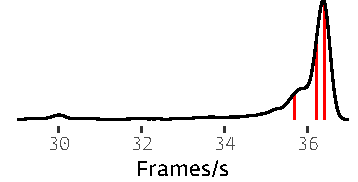
\includegraphics[]{figures/test_7_fps.pdf}
\caption{Probability density of framerates for 960 x 540px grating rendered at 1080p. Red lines indicate quartiles}
\label{fig:framerate}
\end{marginfigure}

Autopilot is appropriate for realtime rendering of simple stimuli, and the proof-of-concept API we built around Psychopy doesn't impose discernible overhead (Mean framerate for a \texttt{960 x 540px} grating at \texttt{1080p} in Autopilot: \texttt{36.2 fps}, vs. \texttt{timeByFrames}: \texttt{35.0 fps}). In the future we will investigate prerendering and caching complex stimuli in order to increase performance. A straightforward option for higher-performance video would be to deploy an Autopilot agent running on a desktop computer with a high-performance GPU, or to use a single-board computer with a GPU like the \href{https://www.nvidia.com/en-us/autonomous-machines/embedded-systems/jetson-nano/}{NVIDIA Jetson} (\$99)\sidenote{as we did in \citep{kaneRealtimeLowlatencyClosedloop2020a}}.

\begin{table}
\caption{Tests performed over 1000 frames with PsychoPy's \href{https://github.com/psychopy/psychopy/blob/3.1/psychopy/demos/coder/timing/timeByFrames.py}{\texttt{timeByFrames}} test.}
    \begin{tabular}{rrr|rr}
        \toprule
        \textbf{Stimulus} & \textbf{Resolution} & \textbf{Size / \# Dots}& \textbf{Mean FPS} & \textbf{$\sigma$ FPS} \\
        \midrule 
        Gabor Filter & 1280 x 720  & 300 x 300px & 106.4 & 5.5 \\
        Gabor Filter & 1920 x 1080 & 300 x 300px & 75.2 & 3.5\\
        Gabor Filter & 1280 x 720 & 640 x 360px & 53.5 & 2.2\\ 
        Gabor Filter & 1920 x 1080 & 960 x 540px & 35.0 & 1.0 \\
        Gabor Filter & 1280 x 720 & 720 x 720px & 41.5 & 2.2 \\
        Gabor Filter & 1920 x 1080 & 1080 x 1080px & 20.1 & 0.7 \\
        Random Dots & 1280 x 720 & 100 dots & 98.0 & 3.8 \\
        Random Dots & 1920 x 1080 & 100 dots & 67.6 & 3.0 \\
        Random Dots & 1280 x 720 & 1000 dots & 20.9 & 0.25 \\
        Random Dots & 1920 x 1080 & 1000 dots & 19.5 & 0.36 \\
        \bottomrule
    \end{tabular}
    \label{tab:fpstests}
\end{table}
